\chapter{Morphological processes and analogy}\label{chap:structural}

So far we have seen how the analogical relations between nouns reflect the grammatical structuring and type system of the lexicon. A common trait in the previous cases is that the morphological markers have all been suffixes. We also saw that it was only the ending of the stems (and some additional phonological information like the number of syllables and stress placement) that helped as predictors. This kind of correlation is often found in the literature on phonologically conditioned morphology and analogy in general. There are only a handful of studies in which the beginning of words were found to have a conditioning effect on some morphological process \autocite{Bybee.1982, Kopcke.1984}, and studies that examine prefixes are even rarer.

Some well-known phenomena in phono-syntax suggest that this relation might not be coincidental. The choice between \textit{a} and \textit{an} in English, or the choice between \textit{la} and \textit{el} in Spanish (in Spanish feminine nouns can use the masculine definite article \textit{el} if they begin with a stressed /a/, see \citealt{Harris.1987}), are conditioned by the first segment of the following word. This makes intuitive sense, but it is not obvious why it should be the case. It would be perfectly possible that suffix selection depended on the first segment of the stem, or the second vowel, etc.

To explore this question I look at three different phenomena in this chapter: Swahili noun classes, Otomi verb classes and Hausa plurals. Swahili and Otomi are relevant to the overall question of this chapter because they use prefixes instead of suffixes, and Hausa has complex plural formations. %complete

\section{Prefixes and gender: Swahili noun classes}

\is{Prefixation|(}
\il{Swahili|(}

Swahili, like other Bantu languages, has a noun class 
system in which all nouns belong to a specific, partially conditioned, class. Traditional Swahili grammars list eleven main classes for Swahili nouns, which are presented in \tabref{tab:swahili-classes}.\footnote{I have omitted classes 14 (abstractions), 15 (verbal infinitives) and 16-18 (locatives). For classes 9 and 10, \textit{N} represents three possible markers: \textit{n-}, \textit{ny-} or \textit{m-}.} These classes are defined by a prefix on the noun and can mark either singular or plural. For the most part, noun classes are lexically determined, with a few classes being determined by derivational morphemes (diminutives, etc.). %complete

\begin{table}
  \centering
  \begin{tabular}{lll}
    \lsptoprule
    class & form                   & number   \\
    \midrule
    1     & m-                     & singular \\
    2     & wa-                    & plural   \\
    3     & m-                     & singular \\
    4     & mi-                    & plural   \\
    5     & $\varnothing \sim$ ji- & singular \\
    6     & ma-                    & plural   \\
    7     & ki-                    & singular \\
    8     & vi-                    & plural   \\
    9     & N-                     & singular \\
    10    & N-                     & plural   \\
    11    & u-                     & singular \\
    \lspbottomrule
  \end{tabular}\caption{Swahili noun classes}\label{tab:swahili-classes}
\end{table}

\textcite{Corbett.1991}, however, suggests that Swahili noun classes should be treated as genders, not very differently from other gender systems. The reason is that all the properties of a gender system are present in the Swahili class system, like agreement with determiners and adjectives as shown in \REF{swahili-class-exe}.\footnote{The examples in this section are taken from \textcite{Corbett.1991}, who in turn takes them from \textcite[159-183]{Welmers.1973}.}

\begin{exe}
    \ex \label{swahili-class-exe}
    \gll \textit{ki}-kapy \textit{ki}-kubwa \textit{ki}-moja \textit{ki}-lianguka\\
    \textsc{cl7}-basket \textsc{cl7}-large \textsc{cl7}-one \textsc{cl7}-fell\\
    \glt `One large basket fell.'
\end{exe}

The class marker \textit{ki} agrees with the verb, noun, adjective and determiner, just like German adjectives agree with their nouns. The fact that these are genders can be seen more clearly from cases where the prefix on a noun is `wrong', in the sense that it usually denotes some other class than what it is actually agreeing with. In \REF{swahili-class-exe-cl2} \autocite[45]{Corbett.1991} we see for example (a) that \textit{tu} (`person') takes a marker for class 1, while the agreement with the verb is the marker of class 2. A similar situation arises in example (b) where there seems to be a disagreement between the different markers. For this reason \textcite{Corbett.1991} argues that there are two different system: inflection class and gender proper.

\begin{exe}
    \ex
    \begin{xlist}
        \ex \label{swahili-class-exe-cl1}
        \gll \textit{m}-tu \textit{wa}-mepotea\\ 
         \textsc{cl1}-person \textsc{cl2}-is.missing\\
        \glt `A parson is missing.'
        \ex \label{swahili-class-exe-cl2}
        \gll \textit{ki}-faru \textit{m}-dogo \textit{wa}-likuwa hapa\\
         \textsc{cl7}-rhinoceros \textsc{cl1}-small \textsc{cl2}-was here\\
        \glt `A small rhinoceros was here.'
    \end{xlist}
\end{exe}

Thus, grouping the singular and plural forms we get the six genders (the  original proposal in \textcite[47]{Corbett.1991} suggests seven) in \tabref{tab:genders-swahili}.

\begin{table}
  \centering
  \begin{tabular}{lll}
    \lsptoprule
    Class & Prefix on noun             & Verbal agreement \\
    \midrule
    1/2   & m-/wa-                     & a-/wa-           \\
    3/4   & m-/mi-                     & u-/i-            \\
    5/6   & $\varnothing \sim$ ji-/ma- & li-/ya-          \\
    7/8   & ki-/vi-                    & ki-/vi-          \\
    9/10  & N-/N-                      & i-/zi-           \\
    11/10 & u-/N-                      & u-/zi-           \\
    \lspbottomrule
  \end{tabular}
  \caption{Swahili genders}\label{tab:genders-swahili}
\end{table}

Swahili has received some attention with respect to how nouns are assigned to a given gender. \textcite[47]{Corbett.1991} suggests that ``for Swahili we require semantic and morphological assignment rules''. The author lists (p. 47) the following rules (adapted) to account for how nouns are assigned to their gender class in Swahili. When in conflict, the semantic rules override the morphological rules:\\

\noindent
Semantic assignment:

\begin{enumerate}
  \item augmentatives belong to gender 5/6
  \item diminutives belong to gender 7/8
  \item remaining animates belong to gender 1/2
\end{enumerate}

\noindent
Morphological assignment:

\begin{enumerate}
  \item morphological class 3/4 (m-/mi-) $\rightarrow$ gender 3/4
  \item morphological class 5/6 ($\varnothing \sim$ ji-/ma-) $\rightarrow$ gender 5/6
  \item morphological class 7/8 (ki-/vi-) $\rightarrow$ gender 7/8
  \item morphological class 9/10 (N-/N-) $\rightarrow$ gender 9/10
  \item morphological class 11/10 (u-/N-) $\rightarrow$ gender 11/10
\end{enumerate}

\textcite[48]{Corbett.1991} also provides some additional semantic regularities: plants are often in gender 3/4, fruits in gender 5/6, animals in gender 9/10 and small objects in gender 7/8. This list is further expanded by \textcite{Contini-Morava.1994}, who provides strong additional semantic grounding for most of the six genders.

With all these rules combined, we have a system where we expect that phonological analogies will be rather weak. Because of its heavy semantic component, and because speakers are usually quite certain with regards to inflectional class assignment upon encountering a noun, the need for analogical relations is greatly reduced.

\subsection{Materials}

I compiled a list of Swahili nouns with their corresponding classes by combining the list given in the Wiktionary page for Swahili \autocite{WikimediaFundation.2016}, and extracting all the nouns for which class information is available in the \textit{Mgombato: Digo-English-Swahili Dictionary} \autocite{Mwalonya.2004}. Because the extraction from the Swahili dictionary relied on optical character recognition, there is some degree of noise in the data. I removed all clear errors of nouns containing punctuation marks. The result is 3081 nouns, distributed as shown in \figref{fig:class-freq-swahili}. There were not enough \textit{u-} marked nouns to properly work with the 11/10 gender.

\begin{figure}
  \centering
  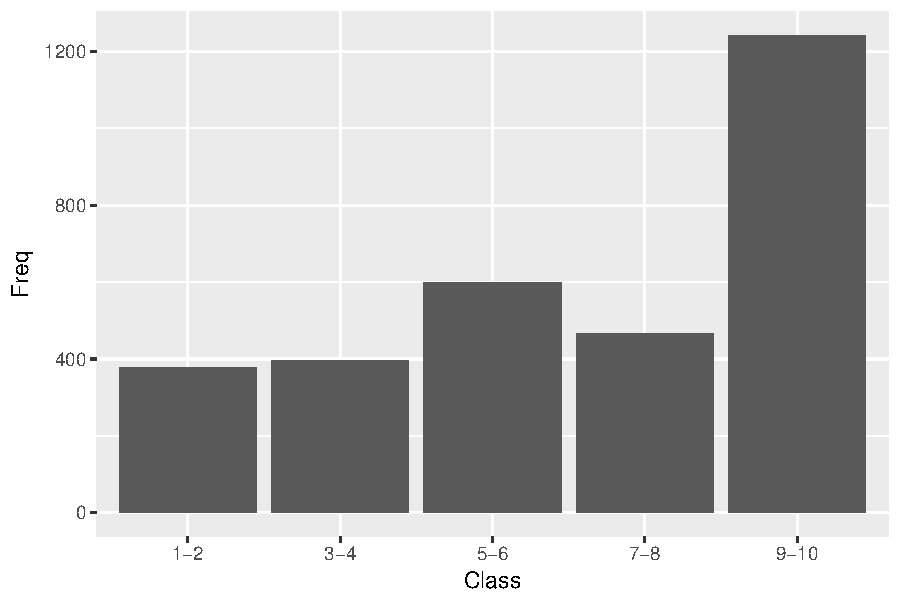
\includegraphics[width=0.7\textwidth]{./figures/swahili/freq-plot.pdf}
  \caption{Type frequency of Swahili genders}\label{fig:class-freq-swahili}
\end{figure}

Because the classes are uneven in terms  of members, models including the whole data-set tended to under-perform\footnote{The reason is that the neural network models are sensitive to type frequency. This is not very important if the predictors are strong enough, but in cases where the predictors are weak, the model tries to optimize for general accuracy, and over-predicts the most frequent class.}. To control for this, I randomly extracted 378 nouns for each class (the size of the smallest class in the original data-set). This produced a final data-set with 1890 nouns in total.

In terms of pre-processing, Swahili has a series of digraphs (e.g. \textit{mb} $\rightarrow$ /$^m$b/), which I converted into single character representations to aid the analogical model. Otherwise, this is a relatively poor data-set in terms of features. We do not have any extra semantic or morphological information to aid the models.

\subsection{Results}

In our first model we investigate whether the first and second segments of the stem (that is, after removing the class prefixes) can predict to any degree the inflectional class of Swahili nouns with the model \texttt{class $\sim$ first.1 + first.2}.\footnote{With 0 hidden nodes and a decay rate of 0.1. A more complex model with interactions did not perform any better.} The results, shown in \tabref{tab:class-swa} and \tabref{tab:class-swa-stats}, are not very good in themselves. The accuracy is barely above chance, and the kappa score is very small. This basically means that there is very little information about inflection class just in the phonological shape of the stem. But this result is not really surprising. Swahili speakers encounter nouns with the prefix or some agreeing forms, and there is little ambiguity about their class.

\begin{table}
  \centering
  \begin{tabular}{rrrrrr}
    \lsptoprule
    \multicolumn{6}{c}{Reference}             \\
    \midrule
    Prediction & 1-2 & 3-4 & 5-6 & 7-8 & 9-10 \\
    1-2        & 155 & 96  & 47  & 69  & 46   \\
    3-4        & 85  & 130 & 48  & 78  & 63   \\
    5-6        & 44  & 49  & 168 & 84  & 74   \\
    7-8        & 44  & 53  & 46  & 92  & 49   \\
    9-10       & 50  & 50  & 69  & 55  & 146  \\
    \lspbottomrule
  \end{tabular}
  \caption{Confusion Matrix for the model predicting inflection class of Swahili nouns}\label{tab:class-swa}
\end{table}

\begin{table}
  \centering
  \begin{tabular}{lllrrr}
    \lsptoprule
    \multicolumn{6}{c}{Overall statistics:} \\

    \midrule
    \multicolumn{6}{c}{Accuracy: 0.3656}            \\
    \multicolumn{6}{c}{95\% CI: (0.3439, 0.3878)}   \\
    \multicolumn{6}{c}{No Information Rate: 0.2} \\
    \multicolumn{6}{c}{Kappa: 0.2}               \\
    \lspbottomrule
  \end{tabular}
  \caption{Overall statistics for Confusion Matrix in \tabref{tab:class-swa}}\label{tab:class-swa-stats}
\end{table}

Next, we compare this model to one where we use the endings of the nouns instead of the initial segments, as shown in \tabref{tab:class-swa-last}. In this model we see performance at chance level.

\begin{table}
  \centering
  \begin{tabular}{rrrrrr}
    \lsptoprule
    \multicolumn{6}{c}{Reference}             \\
    \midrule
    Prediction & 1-2 & 3-4 & 5-6 & 7-8 & 9-10 \\
    1-2        & 195 & 94  & 92  & 89  & 102  \\
    3-4        & 35  & 91  & 71  & 79  & 43   \\
    5-6        & 32  & 49  & 54  & 40  & 58   \\
    7-8        & 31  & 68  & 67  & 91  & 54   \\
    9-10       & 85  & 76  & 94  & 79  & 121  \\
    \lspbottomrule
  \end{tabular}
  \caption{Confusion Matrix for the model predicting inflection class of Swahili nouns}\label{tab:class-swa-last}
\end{table}

\begin{table}
  \centering
  \begin{tabular}{lllrrr}
    \lsptoprule
    \multicolumn{6}{c}{Overall statistics:} \\
    \midrule
    \multicolumn{6}{c}{Accuracy: 0.2921}            \\
    \multicolumn{6}{c}{95\% CI: (0.2716, 0.3131)}   \\
    \multicolumn{6}{c}{No Information Rate: 0.2} \\
    \multicolumn{6}{c}{Kappa: 0.1151}               \\
    \lspbottomrule
  \end{tabular}
  \caption{Overall statistics for Confusion Matrix in \tabref{tab:class-swa-last}}\label{tab:class-swa-last-stats}
\end{table}

Finally, we try a model that combines the first two segments of the noun, the last segment, and length in letters with the formula: \texttt{class $\sim$ final.1 + first.1 + first.2 + length}. The results are presented in \tabref{tab:class-swa-last-first} and \tabref{tab:class-swa-last-first-stats}. This model shows a slight improvement from the model only using the first segments.


\begin{table}
  \centering
  \begin{tabular}{rrrrrr}
    \lsptoprule
    \multicolumn{6}{c}{Reference}             \\
    \midrule
    Prediction & 1-2 & 3-4 & 5-6 & 7-8 & 9-10 \\
    1-2        & 178 & 83  & 49  & 42  & 73   \\
    3-4        & 68  & 158 & 47  & 86  & 60   \\
    5-6        & 44  & 43  & 164 & 91  & 58   \\
    7-8        & 25  & 55  & 56  & 105 & 40   \\
    9-10       & 63  & 39  & 62  & 54  & 147  \\
    \lspbottomrule
  \end{tabular}
  \caption{Confusion Matrix for the model predicting inflection class of Swahili nouns}\label{tab:class-swa-last-first}
\end{table}

\begin{table}
  \centering
  \begin{tabular}{lllrrr}
    \lsptoprule
    \multicolumn{6}{c}{Overall statistics:} \\
    \midrule
    \multicolumn{6}{c}{Accuracy: 0.3979}            \\
    \multicolumn{6}{c}{95\% CI: (0.3757, 0.4204)}   \\
    \multicolumn{6}{c}{No Information Rate: 0.2} \\
    \multicolumn{6}{c}{Kappa: 0.2474}               \\
    \lspbottomrule
  \end{tabular}
  \caption{Overall statistics for Confusion Matrix in \tabref{tab:class-swa-last-first}}\label{tab:class-swa-last-first-stats}
\end{table}

\clearpage 
The overall evaluation of this final model can be seen in \figref{fig:overall-fi-class-sg-swahili}. 
This figure basically shows that the main effect comes from the first segment, but that the other factors still play a minor role.

\begin{figure}
  \centering
  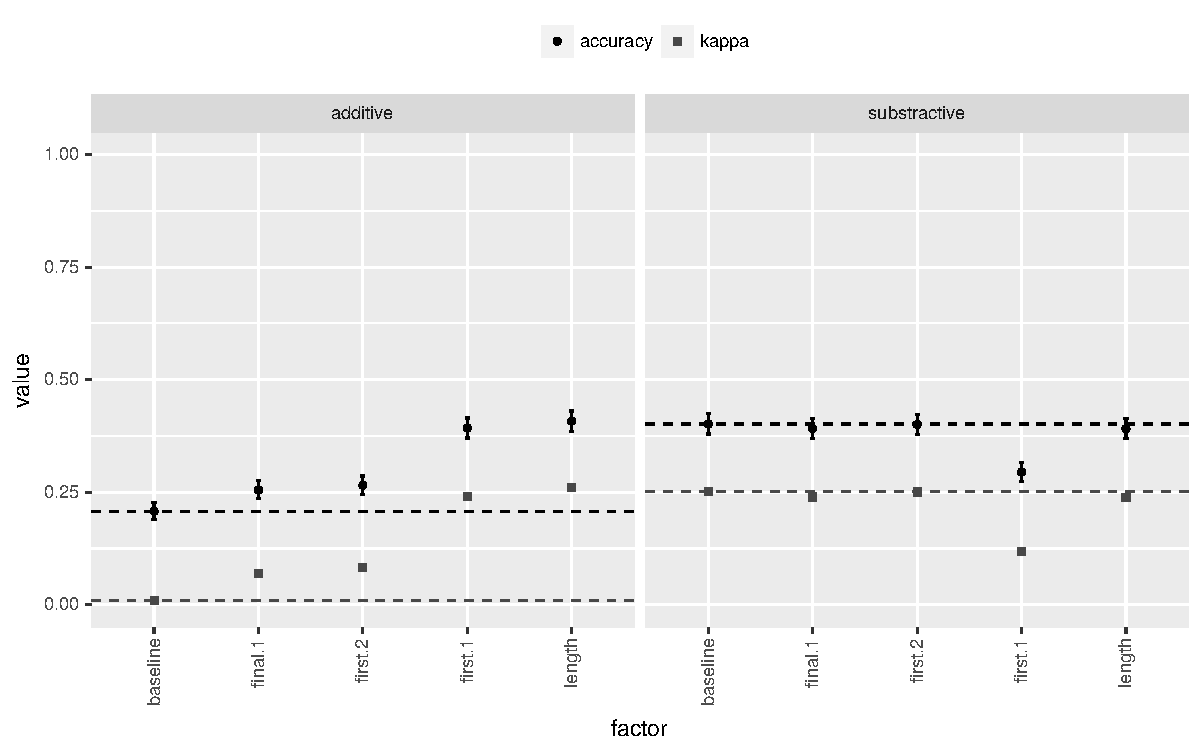
\includegraphics[width=1.0\textwidth]{./figures/swahili/p-fi-overall.pdf}
    \caption{Additive (left) and subtractive (right) accuracy and kappa scores for the model predicting gender in Swahili}\label{fig:overall-fi-class-sg-swahili}
\end{figure}

The model including both beginning and ending of the nouns clearly performed better, and even though the main effect came from the beginning of the nouns, the ending did play a role.

It is possible that the current analogical relations of the Swahili noun classes are the product of some previous more regular system \autocite{Nurse.1993}, and not of actual productive schemas speakers use. Because the analogical effects are so weak, the most likely explanation in this case is that the semantic component is much stronger, and thus phonological analogy is not as important for speakers. The important point here is that we do see a stronger effect of the beginning of the stem 
than of the ending of the stem.

\il{Swahili|)}
\is{Prefixation|)}

\section{Prefixes and inflection classes: Eastern Highland Otomi}

\il{Highland Otomi|(}

\subsection{Verb classes in Eastern Highland Otomi}

Eastern Highland Otomi (Otomi from now on) is a Mesoamerican language of the Otoman\-guean family spoken in Mexico \autocite{Echegoyen.1979}. The Otomi verb system is relevant for the proposal in this book because, like in Swahili, it has inflection classes where the actual inflection is produced by a prefix instead of a suffix.

% Otomí orthography has 13 vowels and 20 consonants. ʉøëẹạ aeiou
The verbs are organized in four classes according to \textcite{Echegoyen.1979}, and five classes according to \textcite{Feist.2015}. Examples of these classes can be found in \tabref{tab:class-otomi}.

\begin{table}
    \centering
    \footnotesize
  \begin{tabular}{lllllll}
    \lsptoprule
                 &     & Class I.a & Class I.b       & Class II     & Class III      & Class IV      \\
                 &     & `gather'  & `save'          & `walk'       & `fix'          & `hurry'       \\
    \midrule
    Incompletive & 1st & dí joni   & dí -n yäni      & dí 	’yo & dí -dí hoki    & dí -dí xøni   \\
                 & 2nd & gí joni   & gí -n yäni      & gí 	’yo & gí -dí hoki    & gí -dí xøni   \\
                 & 3rd & (i) joni  & i -n yäni       & (i) 	’yo & (i) -di hoki   & (i) -di xøni  \\
    \midrule
    Imperfect    & 1st & dmí joni  & dmí -n yäni     & dmí 	’yo & dmí -dí hoki   & dmí -dí xøni  \\
                 & 2nd & gmí joni  & gmí -n yäni     & gmí 	’yo & gmí -dí hoki   & gmí -dí xøni  \\
                 & 3rd & mí joni   & mí -n yäni      & mí 	’yo & mí -dí hoki    & mí -dí xøni   \\
    \midrule
    Completive   & 1st & dá joni   & dá 	yäni & dá -n ’yo    & dá 	hoki & dá -n xøni    \\
                 & 2nd & gá joni   & gá 	yäni & gá -n ’yo    & gá 	hoki & gá -n xøni    \\
                 & 3rd & bi goni   & bi 	yäni & bi -n ’yo    & bi 	hoki & bi -n xøni    \\
    \midrule
    Perfect      & 1st & xtá joni  & xtá 	yäni & xtá -n ’yo   & xtá 	hoki & xtá -n xøni   \\
                 & 2nd & xká joni  & xká 	yäni & xká -n ’yo   & xká 	hoki & xká -n xøni   \\
                 & 3rd & xø-n goni & xø -n yäni      & xø -n ’yo    & xø 	hoki & xø -n xøni    \\
    \midrule
    Pluperfect   & 1st & xtá joni  & xtá 	yäni & xtá -n ’yo   & xtá 	hoki & xtá -n xøni   \\
                 & 2nd & xkí joni  & xkí 	yäni & xkí -n ’yo   & xkí 	hoki & xkí -n xøni   \\
                 & 3rd & xí goni   & xí 	yäni & xí -n ’yo    & xí 	hoki & xí -n xøni    \\
    \midrule
    Irrealis     & 1st & ga joni   & ga -n yäni      & da -n ’yo    & ga 	hoki & da -n xøni    \\
                 & 2nd & gi joni   & gi -n yäni      & ga -n ’yo    & gi 	hoki & ga -n xøni    \\
                 & 3rd & da goni   & da 	yäni & di -n ’yo    & da 	hoki & di -n 	xøni \\
    \lspbottomrule
  \end{tabular}
  \caption{Otomi inflection classes}\label{tab:class-otomi}
\end{table}

Capturing the class system in Otomi requires positing five independent types, but nonetheless there is a degree of organization between these types. The important thing to observe here is that classes \textit{III} and \textit{IV} share an extra \textit{-di-} segment in the incompletive and imperfect, while classes \textit{I} and \textit{II} do not have this feature. Meanwhile, class \textit{II} and class \textit{IV} share the use of an extra \textit{-n} in the completive, perfect, pluperfect and irrealis. Class \textit{I.a} can either be grouped with classes \textit{I.b} and \textit{III} or as a completely independent class, depending on the property involved.

\subsection{Materials}

For this case study I used the inflection class database by \textcite{Feist.2015} (based on \citealt{Echegoyen.1979}, \citealt{Echegoyen.2007} and \citealt{Voigtlander.2007}). This database contains 1998 verbs, all of which were analyzed and assigned to one of the five classes. It also contains information about whether the verb is transitive or not, its stem and citation form. I performed no extra processing on the data and used it as it was.

\subsection{Results}

In terms of complexity, the model for Otomi is probably the one with the most factors. As predictors, I included the first three segments (with an interaction between the first and second segment), the last two segments, the tone of the citation form, and whether the verb is transitive or not: \texttt{class $\sim$ first.1 * first.2 + first.3 + Transitivity + last.1 + last.2 + tone}.\footnote{The model contained no hidden nodes and a decay rate of 0.1.} The confusion matrix for this model is shown in \tabref{tab:class-otomi-cm} and the accuracy measures in \tabref{tab:class-otomi-stats}.

\begin{table}
  \centering
  \begin{tabular}{lrrrrr}
    \lsptoprule
               & Reference                  \\
    \midrule
    Prediction & Ia  & Ib & II  & III & IV  \\
    Ia         & 609 & 6  & 46  & 141 & 56  \\
    Ib         & 6   & 29 & 2   & 8   & 0   \\
    II         & 50  & 2  & 284 & 27  & 85  \\
    III        & 82  & 15 & 10  & 249 & 14  \\
    IV         & 36  & 3  & 74  & 28  & 136 \\
    \lspbottomrule
  \end{tabular}
    \caption{Confusion matrix for the model predicting inflection class in Otomi}
  \label{tab:class-otomi-cm}
\end{table}

We see that classes are mostly predictable for Otomi, but there is some degree of confusion. The accuracy metrics show that \textit{class-Ia} is receiving most of the miss-classifications, which is to be expected, this being the most frequent class. Interestingly, \textit{class-Ib} is only mildly confused with \textit{class-Ia}, and much more confused with \textit{class-III}.

\begin{table}
  \centering
  \begin{tabular}{rlllll}
    \lsptoprule
    \multicolumn{6}{c}{Overall Statistics}                                         \\
    \midrule
    \multicolumn{6}{c}{Accuracy : 0.6542}                                          \\
    \multicolumn{6}{c}{95\% CI : (0.6328, 0.675)}                                  \\
    \multicolumn{6}{c}{No Information Rate : 0.3919}                               \\
    \multicolumn{6}{c}{Kappa : 0.5211}                                             \\
    \midrule
    \multicolumn{6}{c}{Statistics by Class:}                                       \\
    \midrule
                      & Class: Ia & Class: Ib & Class: II & Class: III & Class: IV \\
    Sensitivity       & 0.7778    & 0.52727   & 0.6827    & 0.5497     & 0.46735   \\
    Specificity       & 0.7951    & 0.99177   & 0.8963    & 0.9217     & 0.91740   \\
    Neg Pred Value    & 0.8474    & 0.98669   & 0.9148    & 0.8747     & 0.90994   \\
    Balanced Accuracy & 0.7864    & 0.75952   & 0.7895    & 0.7357     & 0.69238   \\
    \lspbottomrule
  \end{tabular}
  \caption{Accuracy scores for \tabref{tab:class-otomi-cm}}\label{tab:class-otomi-stats}
\end{table}


The important fact regarding Otomi is the relative effects of the different factors. In Swahili we saw that both the first segments and final segment of the nouns carried some information about gender. In this case, we have more or less the same situation. \figref{fig:fact-imp-otomi} shows the additive and subtractive model evaluation plots. On the left, we see that all factors used provide small increases to model performance. Moreover, on the right, we see that the two most important factors were the interaction between the first two segments of the verb and the verb's transitivity. The interesting thing to note is that the first segments were much more important for predicting inflection class than the final segments.

\begin{figure}
  \centering
  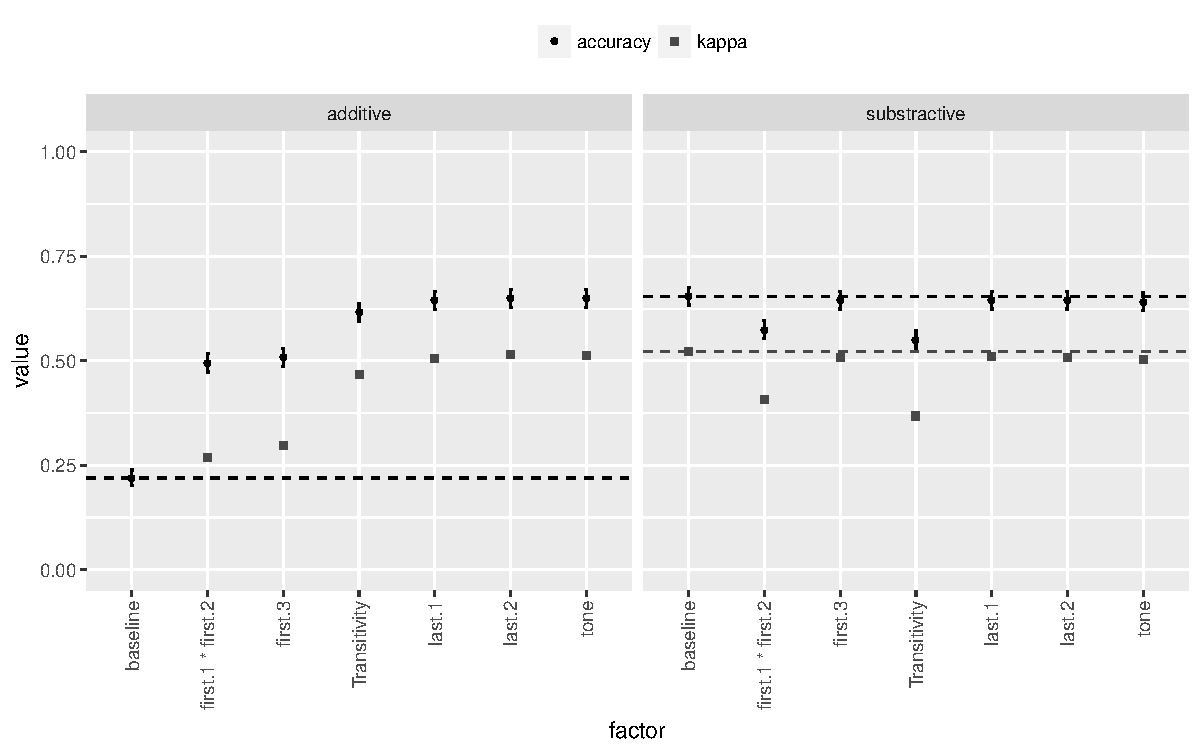
\includegraphics[width=0.9\textwidth]{./figures/otomi/fact-imp.pdf}
  \caption{Additive (left) and subtractive (right) accuracy and kappa scores for the model predicting inflection class}\label{fig:fact-imp-otomi}
\end{figure}

Once more, classes that trigger prefixing processes are predictable from analogies based on the beginning of words, much more so than analogies based on the endings. The fact that the endings did play a minor role is interesting. It probably means that both Otomi and Swahili are susceptible to word size schemas, similar to how in German nouns gender is determined by both initial and final segments \autocite{Kopcke.1984}.% Clustering based on similarity may or may not correspond to a possible class hierarchy.

\il{Highland Otomi|)}

\section{Stem changing processes: Hausa plural classes}

\il{Hausa|(}

\subsection{The Hausa plural system}

The Hausa plural system is too complex to be fully explored here, but some of its properties are relevant to the overall theme of this chapter. First, there seems to be little agreement with regards to how many plural classes there are in Hausa, and an analysis could go anywhere between ``many'' \autocite{Migeod.1914}, around thirty \autocite{Schon.1862}, to twenty macro-classes \autocite{Newman.2000}, or the many more sub-classes Newman identifies. For this study I follow the macro-classes defined by \textcite{Newman.2000}, which are given in \tabref{tab:macro-hausa}\footnote{Because the dictionary I use for the data \autocite{Bargery.1951} does not distinguish between the retroflex and rolled \textit{r}, and between long and short vowels, I will not mark these features here. For tone representation I follow \textcite{Newman.2000}, with high tone unmarked, low tone marked with a grave accent, and falling tone with a circumflex accent.}.

\begin{table}
  \centering
  \begin{tabular}{llll}
    \lsptoprule
    Class & Singular & Plural                          & Gloss          \\
    \midrule
    a-a   & sirdì    & sir\textit{à}d\textit{a}        & `saddle'       \\
    a-e   & gulbi    & gul\textit{à}b\textit{e}        & `stream'       \\
    a-u   & kurmì    & kur\textit{à}m\textit{u}        & `grove'        \\
    -aCe  & wuri     & wur\textit{àre}                 & `place'        \\
    -ai   & malàm    & malàm\textit{ai}                & `teacher'      \\
    -anni & watà     & wàt\textit{ànni}                & `moon'         \\
    -awa  & talàkà   & talak\textit{awa}               & `commoner'     \\
    -aye  & zomo     & zom\textit{àye}                 & `hare'         \\
    -Ca   & tabò     & tab\textit{ba}                  & `scar'         \\
    -Cai  & tudù     & tùd\textit{dai}                 & `high ground'  \\
    -ce2  & ciwò     & cìwà\textit{ce}-\textit{cìwàce} & `illness'      \\
    -Cuna & cikì     & cik\textit{kunà}                & `belly'        \\
    -e2   & camfì    & càmf\textit{e}-\textit{càmfe}   & `superstition' \\
    -i    & tàurarò  & tàuràr\textit{i}                & `star'         \\
    -oCi  & tagà     & tag\textit{ogi}                 & `window'       \\
    -u    & kujèra   & kùjèr\textit{u}                 & `chair'        \\
    u-a   & cokàli   & cok\textit{uà}                  & `spoon'        \\
    -uka  & layì     & lay\textit{ukà}                 & `lane'         \\
    -una  & rìga     & rig\textit{unà}                 & `grown'        \\
    X2    & àkàwu    & àkàwu-\textit{àkàwu}            & `clerk'        \\
    \lspbottomrule
  \end{tabular}
  \caption{Hausa plural macro-classes} \label{tab:macro-hausa}
\end{table}

As we can observe in \tabref{tab:macro-hausa}, some plural classes assign their own tonal pattern to the plural forms, independently of the tonal patterns of the singular, while others carry over the tonal pattern of the singular class \autocite[430]{Newman.2000}. There are several reduplication patterns, and several `broken' plurals, where there is a vocalic change before and after the final consonant of the singular. It is worth keeping in mind that these are macro-classes, and one could find an even more fine-grained division, with many subdivisions within each of these classes. Because of this fact, there are no good arguments in favor of a specific hierarchical organization of these classes.

\textcite[chapter 56]{Newman.2000} observes several regularities in the formation of plurals. He mentions, for example, that \textit{-aCe} plurals only occur with CVCVV nouns, while \textit{a-a} plurals tend to appear with CVCCVV nouns (p. 431). Newman gives similar patterns for other macro-classes, but states that ultimately Hausa plurals are not fully predictable.

\subsection{Materials}

I extracted all nouns from \textit{A Hausa-English Dictionary and English-Hausa Vocabulary} by \textcite{Bargery.1951}. The dictionary contains around 3000 nouns, of which only some 1450 have a plural. Of these, quite a few have indications about multiple alternatives. Some of the alternatives are marked as \textit{rare}, or for regional preferences. It is not really possible to work with these overabundant variants \autocites{Migeod.1914, Salim.1981, Newman.2000} because there are just not enough of them (around 150). As a practical solution, I simply took the first variant offered in the dictionary and ignored the rest.
Similarly, in cases where the dictionary offered multiple possible singulars for a noun, I only used the first singular form listed.

Identifying plural classes automatically in Hausa is not a trivial task, and it is not completely clear how many examples fit into \textcite{Newman.2000}'s macro-classes. I followed the definitions as given in \tabref{tab:macro-hausa}. Although this approach is likely to produce some errors, it should mostly give us the right classification. The main difference in the classes I use is that I take four reduplication classes instead of the three listed in \tabref{tab:macro-hausa}: \textit{class-RED-e} and \textit{class-RED-comp} correspond to the \textit{class-X2} and \textit{class-e2} classes identified by \textcite{Newman.2000}. I included \textit{class-RED-id} which consists of cases where the plural is the reduplication of the singular form without additional changes, and a general \textit{class-RED} class with all the cases that do not quite fit into any of the other classes. The \textit{class-ce2} did not have enough members to be usable. Finally, an extra class I include is \textit{class-oi}, which is not explicitly mentioned by \textcite{Newman.2000}, but which had enough members to be distinguished as an independent macro-class. We can see the frequencies of the classes in the data-set in \figref{fig:class-hausa-freqs}.

\begin{figure}
  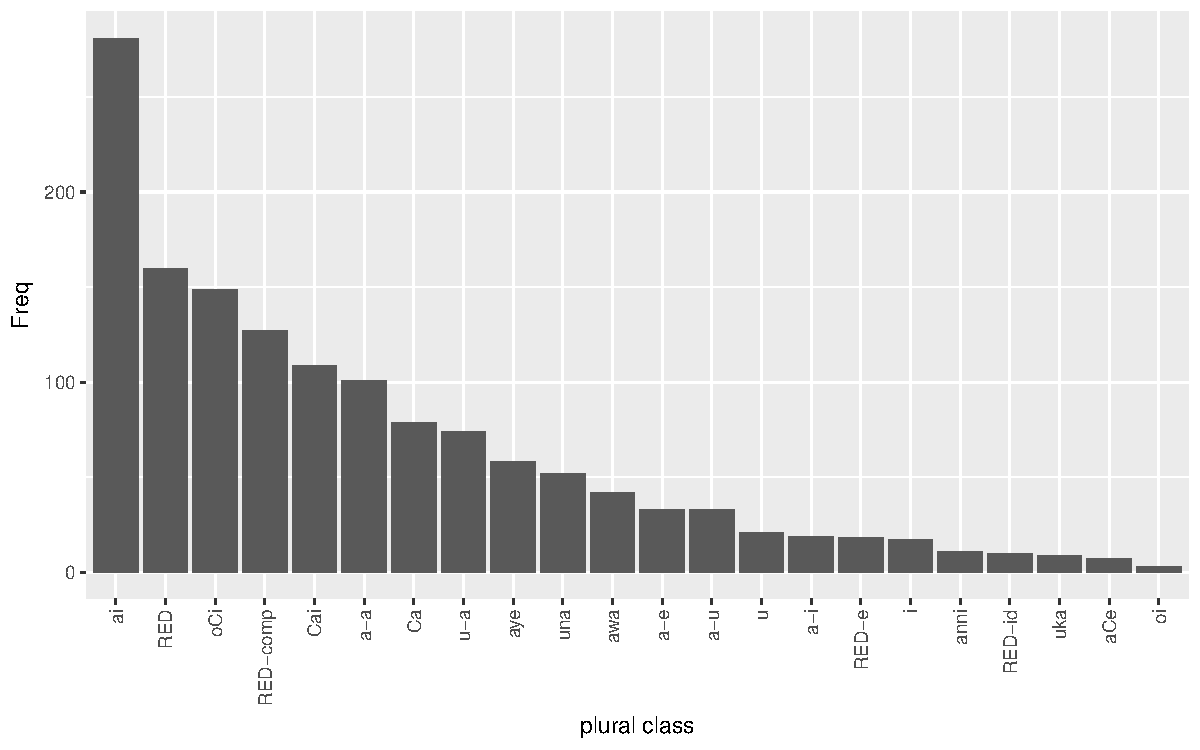
\includegraphics[width=0.9\textwidth]{./figures/hausa/class-freqs.pdf}
  \caption{Type frequency of macro-classes in Hausa}\label{fig:class-hausa-freqs}
\end{figure}

As expected, some classes are considerably more frequent than others, and the general distribution is roughly zipfian. However, it is hard to tell which of these classes are productive, which are irregulars, and which misanalyses.

A serious shortcoming of this database is the lack of information about vowel length. According to Newman (p.c.), several of the macro-classes are strongly correlated with vowel length of the singular, which means there is an important factor missing.

\subsection{Results}

First we look at a model predicting the plural class from structurally defined predictors. Since most of the macro-classes presented in \figref{fig:class-hausa-freqs} are defined by two vowels and a potential consonant between them, I defined the predictors as follows: \texttt{plural class $\sim$ V.1*T.1 + C.1 + V.2 + CVCV.4 + length}.\footnote{The model included one hidden layer with five nodes and a decay rate of 0.1. Gender did not play a significant role in any of the models.} Here, \texttt{V.1} and \texttt{V.2} are the final and prefinal vowels, respectively, \texttt{C.1} is the final consonant, \texttt{T.1} is the final tone of the singular, \texttt{length} the length in letters, and \texttt{CVCV.4} is the CV structure of the final four segments of the singular. In this case, we are specifying an interaction between the final vowel and the tone of that vowel. \textcite[chapter 56]{Newman.2000} makes reference to all these factors, in some way or another, in his analysis of the Hausa plurals. It is therefor no surprise that they play a role in the analogical model.

The results of this model can be seen in \figref{fig:class-hausa-cm} and the corresponding statistics are presented in \tabref{tab:class-hausa-stats}. We see that most classes can be predicted to a relatively high degree of accuracy. There is a clear darker trace along the main diagonal in \figref{fig:class-hausa-cm}, but with some noise for most classes.\footnote{Because the numbers used for shading are log scaled from the actual confusion matrix, the error rates appear slightly higher than they actually are.} In the table there are errors across most classes with no clear structure to them, besides some apparent foci (\textit{class--a-a}, \textit{class--a-e}, \textit{class--ai}, \textit{class--Cai} and \textit{class--oCi}). The accuracy statistics do reveal that the model is performing well above chance, and that there is a significant analogical relation between these classes.


For comparison, a model that does not specify structural analogy: \texttt{plural class $\sim$ final.1*T.1 + final.2 + final.3 + CVCV.4 + length}\footnote{The model included no hidden nodes and a decay rate of 0.1.}, can be seen in \tabref{tab:class-hausa-stats-2}. It is not surprising that this model also performs relatively well, after all, the predictor \texttt{final.1} captures the same information as the predictor \texttt{V.1}.
\largerpage


\begin{figure}[h!]
  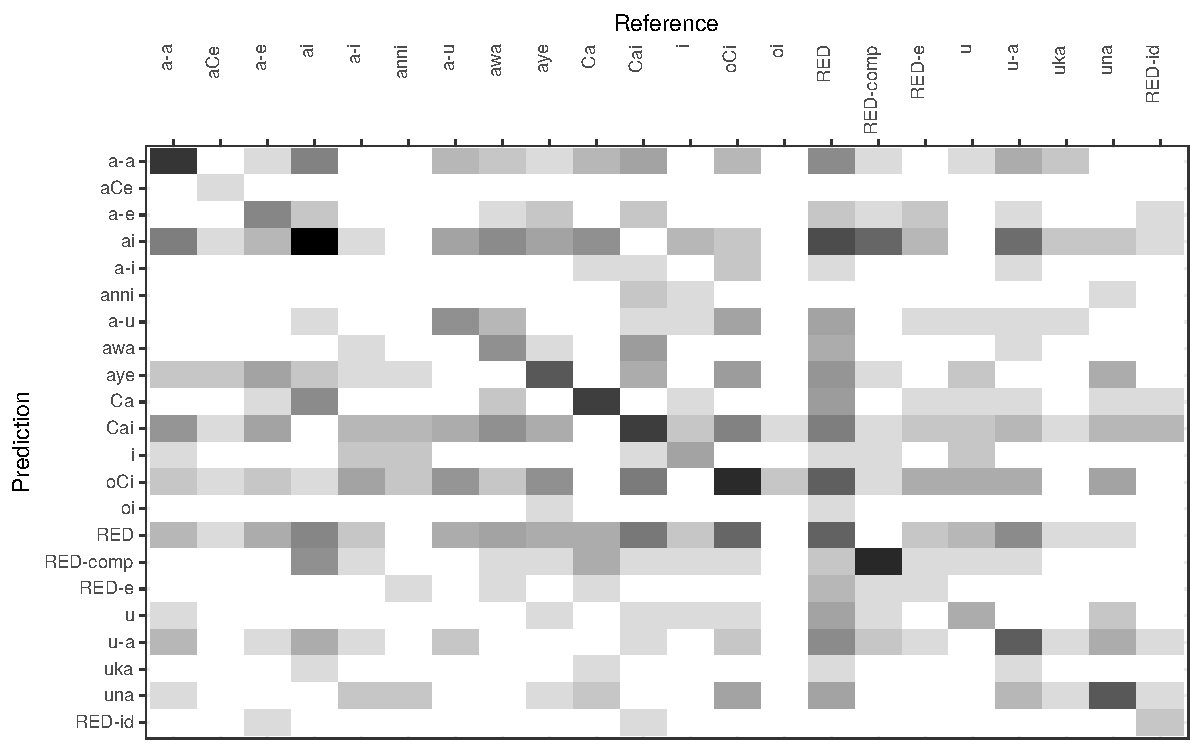
\includegraphics[width=0.9\textwidth]{./figures/hausa/plurals-cm.pdf}
  \caption{Heatmap for the model predicting plural forms in Hausa}\label{fig:class-hausa-cm}
\end{figure}

\begin{table}[h!]
  \centering
  \begin{tabular}{rl}
    \toprule
    \multicolumn{2}{c}{Overall Statistics}                                         \\
    \midrule
    \multicolumn{2}{c}{Accuracy : 0.5425}                                          \\
    \multicolumn{2}{c}{95\% CI : (0.5161, 0.5686)}                                  \\
    \multicolumn{2}{c}{No Information Rate : 0.2082}                               \\
    \multicolumn{2}{c}{Kappa : 0.488}                                             \\
    \bottomrule
  \end{tabular}
  \caption{Accuracy scores for \figref{fig:class-hausa-cm}}\label{tab:class-hausa-stats}
\end{table}

\begin{table}[h!]
  \centering
  \begin{tabular}{rl}
    \lsptoprule
    \multicolumn{2}{c}{Overall Statistics}                                         \\
    \midrule
    \multicolumn{2}{c}{Accuracy : 0.5057}                                          \\
    \multicolumn{2}{c}{95\% CI : (0.5792, 0.5321)}                                  \\
    \multicolumn{2}{c}{No Information Rate : 0.2082}                               \\
    \multicolumn{2}{c}{Kappa : 0.4516}                                             \\
    \lspbottomrule
  \end{tabular}
  \caption{Accuracy scores for the non-structurally defined model}\label{tab:class-hausa-stats-2}
\end{table}
\clearpage 

We can compare model performance for both models (\figref{fig:struc-overall} and \figref{fig:nostruc-overall}). These evaluations reveal that indeed \texttt{final.1} and \texttt{V.1} have more or less the same impact on the model, but for the non-structurally defined model all other predictors become rather insignificant in the subtractive evaluation. The segments captured by both models are the same, but the additional structure does clearly play a role.

\begin{figure}
    \centering  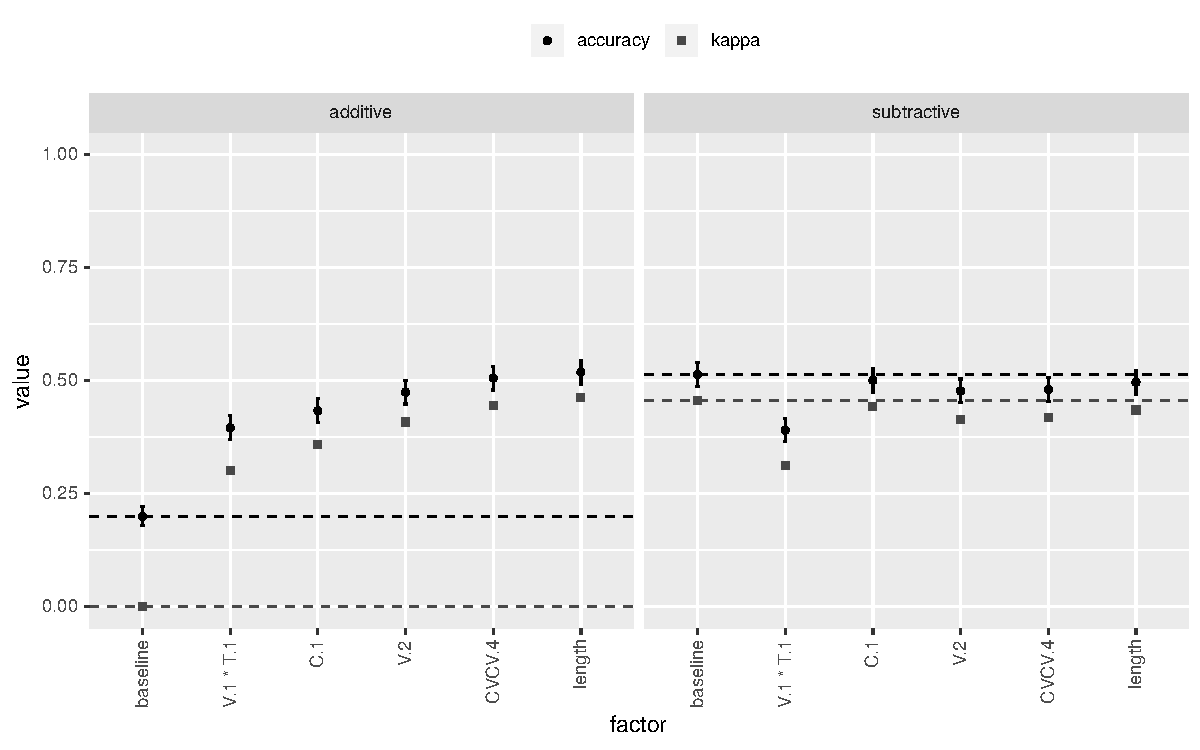
\includegraphics[width=0.9\textwidth]{./figures/hausa/struc-overall.pdf}
    \caption{Additive (left) and subtractive (right) accuracy and kappa scores for the structurally defined model}\label{fig:struc-overall}
\end{figure}

\begin{figure}
    \centering
    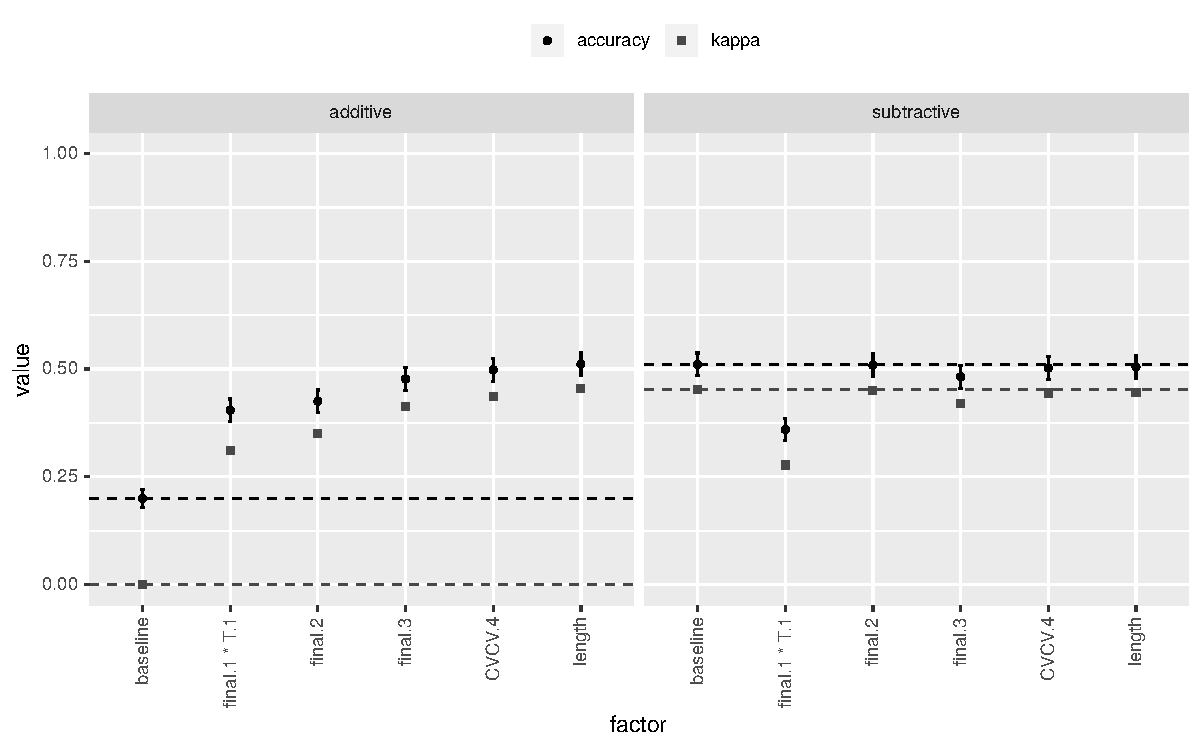
\includegraphics[width=0.9\textwidth]{./figures/hausa/nostruc-overall.pdf}
    \caption{Additive (left) and subtractive (right) accuracy and kappa scores for the non-structurally defined model}\label{fig:nostruc-overall}
\end{figure}

We can also see that the more structural predictors not only achieve a higher accuracy, but also have more independent weights (higher in accuracy in the subtractive evaluations). The main factors are clearly the vowels (and their interaction with tone), while the consonant has less influence. This strongly matches the broken plurals we see in Hausa, where the consonant remains stable and the vowels before and after it are changed.

\il{Hausa|)}

\section{Interim conclusion}

In this chapter I have provided some evidence for a different aspect of analogical models, namely the fact that the analogical specifications, or the points where the analogy takes place, can be related to the actual morphological process. In Swahili and Otomi we see that a prefixing system triggers analogy mostly at the beginning of words, and in Hausa we see how the analogical relation requires a specification that is similar to the actual structure of some plural classes. The results of this chapter should be taken only as a starting point. Two languages for prefixes is too small a sample to draw any definitive conclusions. As mentioned in Part I, this problem had already been raised before:

\begin{quotation}
  The problem faced in the full elaboration of such models, however, is in specifying the relevant features upon which similarity is measured. This is a pressing empirical problem. We need to ask, why are the final consonants of the strong verbs more important than the initial ones? \autocite[62]{Bybee.2010}
\end{quotation}

\noindent
This observation is very difficult to explain from a formal perspective. Assuming the model introduced in Part I is right, there is no way for the hierarchy to `know' what kind of morphological process is being carried out on the different types, and to link that to the inheritance of analogical constraints. From a usage-based perspective, however, these results make more sense. A potential explanation is that speakers are more focused on finding similarities between words where the important changes happen, i.e., the segments before a suffix or after a prefix. This would also explain why there seems to be a distance effect from the edge in most of the other languages, that is, the very last segment tends to be more important than the second to last and so on (though not always). A possible advantage of this explanation is that it also helps reduce the search space for speakers. Unless there was some innate constraint that specified where to look for analogies, speakers would have to analogize over all segments of all stems. The fact that analogies seem to be mostly constrained to the edge of the stem where the morphological process happens, helps reduce the amount of information that has to be considered. This variability of the `where' of the analogy is an advantage for speakers of the language and not a drawback.

%%% Local Variables:
%%% mode: latex
%%% TeX-master: "../main"
%%% End:
